\documentclass{article}

\usepackage[12pt]{extsizes}
\usepackage[T2A]{fontenc}
\usepackage[utf8]{inputenc}
\usepackage[english, russian]{babel}

\usepackage{mathrsfs}
\usepackage[dvipsnames]{xcolor}

\usepackage{amsmath}
\usepackage{amssymb}
\usepackage{amsthm}
\usepackage{indentfirst}
\usepackage{amsfonts}
\usepackage{enumitem}
\usepackage{graphics}
\usepackage{tikz}
\usepackage{tabu}
\usepackage{diagbox}
\usepackage{hyperref}
\usepackage{mathtools}
\usepackage{ucs}
\usepackage{lipsum}
\usepackage{geometry} % Меняем поля страницы
\usepackage{fancyhdr} % Headers and footers
\newcommand{\range}{\mathrm{range}}
\newcommand{\dom}{\mathrm{dom}}
\newcommand{\N}{\mathbb{N}}
\newcommand{\R}{\mathbb{R}}
\newcommand{\E}{\mathbb{E}}
\newcommand{\D}{\mathbb{D}}
\newcommand{\M}{\mathcal{M}}
\newcommand{\Prime}{\mathbb{P}}
\newcommand{\A}{\mathbb{A}}
\newcommand{\Q}{\mathbb{Q}}
\newcommand{\Z}{\mathbb{Z}}
\newcommand{\F}{\mathbb{F}}
\newcommand{\CC}{\mathbb{C}}

\DeclarePairedDelimiter\abs{\lvert}{\rvert}
\DeclarePairedDelimiter\floor{\lfloor}{\rfloor}
\DeclarePairedDelimiter\ceil{\lceil}{\rceil}
\DeclarePairedDelimiter\lr{(}{)}
\DeclarePairedDelimiter\set{\{}{\}}
\DeclarePairedDelimiter\norm{\|}{\|}

\renewcommand{\labelenumi}{(\alph{enumi})}

\newcommand{\smallindent}{
    \geometry{left=1cm}% левое поле
    \geometry{right=1cm}% правое поле
    \geometry{top=1.5cm}% верхнее поле
    \geometry{bottom=1cm}% нижнее поле
}

\newcommand{\header}[3]{
    \pagestyle{fancy} % All pages have headers and footers
    \fancyhead{} % Blank out the default header
    \fancyfoot{} % Blank out the default footer
    \fancyhead[L]{#1}
    \fancyhead[C]{#2}
    \fancyhead[R]{#3}
}

\newcommand{\dividedinto}{
    \,\,\,\vdots\,\,\,
}

\newcommand{\littletaller}{\mathchoice{\vphantom{\big|}}{}{}{}}

\newcommand\restr[2]{{
    \left.\kern-\nulldelimiterspace % automatically resize the bar with \right
    #1 % the function
    \littletaller % pretend it's a little taller at normal size
    \right|_{#2} % this is the delimiter
}}

\DeclareGraphicsExtensions{.pdf,.png,.jpg}

\newenvironment{enumerate_boxed}[1][enumi]{\begin{enumerate}[label*=\protect\fbox{\arabic{#1}}]}{\end{enumerate}}



\smallindent

\header{Математика}{Матбой}{11 июля 2023}

%----------------------------------------------------------------------------------------

\begin{document}
    \large

    \begin{center}
        \textbf{Праздничный математический бой}
    \end{center}

    \begin{enumerate}[label*=\arabic{enumi}.]

        \item Алиса очень хочет на день рождения найти все многочлены $f(x)$ с целыми коэффициентами такие, что $f(n)$ и $f(2^n)$ взаимно просты при любом натуральном $n$.
        Помогите ей!

        \item Парты в конференц зале в ЦРОДе расположены так, что образуют таблицу $8 \times 8$.
        В момент, когда Тимофей отвернулся, каждый ребенок решил подойти к парте своего друга.
        Чтобы не быть замеченными, ученики дошли лишь до соседней по стороне парты (в таблице $8 \times 8$ каждый попал в соседнюю по стороне клетку).
        Когда преподаватель посмотрел обратно в зал, он заметил, что занято минимально возможное количество парт.
        Сколько парт оказалось занято?

%\item Положительные числа $a, b$ и $c$ удовлетворяют условию $a + b + c + abc = 4$. Докажите, что 
%$$\left(1 + \frac{a}{b} + ca\right)\left(1 + \frac{c}{b} + ab\right)\left(1 + \frac{a}{c} + bc\right) \geqslant 27.$$

        \item Федя записал себе в тетрадку подряд 100 чисел $x_1, x_2, \dots, x_{100}$.
        Вадим заметил, что первое число последовательности равно 1, а $x_{n+m} = 2^{n}x_m+3^{m}x_n$.
        Выясните, чему равно $x_{100}$.

        \item На сторонах $AC$ и $AB$ треугольника $ABC$ лежат точки $D$ и $E$ соответственно.
        Прямые $BD$ и $CE$ пересекаются в точке $S, M$~--- середина отрезка $CS$.
        Прямая $BM$ пересекает отрезок $CD$ в точке $T$.
        Известно, что $BE = ES = 1$ и $CD = DS = 2$.
        Докажите, что $AB = AT$.

        \item После пары по целым и дробным частям Алина очень захотела найти все функции $f: \mathbb{R} \rightarrow \mathbb{R}$ такие, что $f([x]y) = f(x)[f(y)]$.
        Здесь $[x]$ — целая часть числа $x$.
        Помогите ей решить эту задачу!


%\item В остроугольном треугольнике $ABC$ проведены высоты $AM$ и $CN$, которые пересекаются в точке $H$. На описанной окружности треугольника $ABC$ выбрана точка $K$ такая, что $AK \perp KH$. Оказалось, что прямая $AB$ делит отрезок $KH$ пополам. Докажите, что $AC \cdot MN = AN \cdot CM$.

%\item В треугольнике $ABC$ $O$ – центр описанной окружности, $I$ – центр вписанной. Прямая, проходящая через $I$ и перпендикулярная $OI$, пересекает $AB$ в точке $X$, а внешнюю биссектрису угла $C$ – в точке $Y$. В каком отношении $I$ делит отрезок $XY$?

        \item В остроугольном треугольнике $ABC$ проведены высоты $BM$ и $CN$, которые пересекаются в точке $H$.
        На описанной окружности треугольника $ABC$ выбрана точка $K$ такая, что $AK \perp KH$.
        Оказалось, что прямая $AB$ делит отрезок $KH$ пополам.
        Докажите, что $KH =AM$.

        \item Миша разбил квадрат $40 \times 40$ на L-тетраминошки, так как это вторая буква в имени <<Алиса>>.
        Докажите, что Настя сможет жестко провести прямую так, чтобы она разрезала не менее шести тетрамишек на доминошки.

        \item Натуральные числа $p$ и $q$ отличаются на 2.
        Саша утверждает, что числа $p^4 + 4$ и $q^4 + 4$ всегда имеют общий делитель.
        Прав ли он?


    \end{enumerate}
    \begin{center}
        \begin{figure}[h]
            \hfill
            \begin{minipage}[h]{0.1\linewidth}
                \center{
\includegraphics[width=1\linewidth]{img4}}
            \end{minipage}
            \begin{minipage}[h]{0.1\linewidth}
                \center{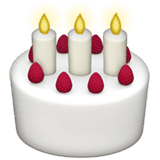
\includegraphics[width=1\linewidth]{img}}
            \end{minipage}
            \begin{minipage}[h]{0.1\linewidth}
                \center{
\includegraphics[width=1\linewidth]{img3}}
            \end{minipage}
            \begin{minipage}[h]{0.4\linewidth}
                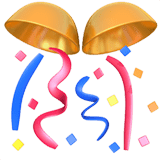
\includegraphics[width=0.25\linewidth]{img2}
            \end{minipage}\label{fig:figure}
        \end{figure}
    \end{center}

%	\begin{minipage}[h]{0.49\linewidth}
%	\end{minipage}
%	\hfill
%	\begin{minipage}[h]{0.49\linewidth}
%		\center{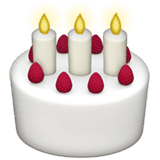
\includegraphics[width=0.5\linewidth]{img.png} \\ б)}
%	\end{minipage}
%	\caption{Зависимость сигнала от шума для данных.}
%	\label{ris:image1}

\end{document}